% !TeX program = lualatex
% !TeX encoding = utf8
% !TeX root = ../Thermod.tex

%=========================================================
\Opensolutionfile{answer}[\currfilebase/\currfilebase-Answers]
\Writetofile{answer}{\protect\section*{\nameref*{\currfilebase}}}
\chapter{Основні поняття. \mbox{Нульовий закон термодинаміки}}\label{\currfilebase}
\makeatletter
\def\input@path{{\currfilebase/}}
\makeatother
%=========================================================

% --------------------------------------------------------
\section{1}
% --------------------------------------------------------

Перший закон термодинаміки не накладає ніяких обмежень щодо взаємного перетворення тепла в роботу і навпаки. Отже, він в принципі не дає відповідь на запитання про напрямок протікання процесів в природі. Також перший закон припускає сценарій, коли камінь, що впав з певної висоти і не пружно ударився об землю, викликав при цьому власне і її нагрівання, може самочинно почати охолоджуватися і підійматися на ту ж висоту, використовуючи при цьому роботу, еквівалентну теплоті, взятій від навколишнього середовища. Ніхто і ніколи не спостерігав подібне і в цьому сенсі теплота не еквівалентна роботі. З іншого боку, неважко навести приклад, коли вся теплота може бути переведена в роботу: ізотермічно нагріваючи ідеальний газ, ми можемо підіймати вантаж. Але при цьому об'єм газу змінюється і в природі залишаються необоротні зміни. З подібними прикладами ми стикаємося кожен день. Наш досвід, вся вікова робота людства вчать, що зокрема: 
\begin{enumerate}
	\item [а)] неможливо ніяким способом обернути процес, при якому тепло виникає завдяки тертю;
	\item [б)] неможливо повністю обернути процес, при якому газ розширюється, не виконуючи над ним роботи і не передаючи тепла ззовні;
	\item [в)] неможливо повністю обернути процеси дифузії і теплопровідності;
	\item [г)] те ж саме можемо сказати про процес вибуху і  багато інших.
\end{enumerate}

Таким чином, існують процеси, необоротні по своїй природі. Важливо, що по закінченню таких процесів, ніяким чином неможливо повернути Природу в попередній стан нічого не змінюючи. Виконуючи таку спробу, ми обов'язково повинні виконати роботу, на виконання якої потрібна деяка кількість теплоти, віднятої у резервуару (наприклад, із допомогою циклу Карно). Таким чином, стан природи буде незворотним чином змінено. Зауважимо, що існування необоротних процесів не витікає логічним чином із якихось теоретичних міркувань; навпаки з механічної точки зору цьому нема пояснення, оскільки всі закони механіки є обернені у часі. Отже, вказані приклади і спостереження – експериментальні факти. Другий закон узагальнює їх, надаючи строге математичне формулювання, дозволяючи на цій основі будувати подальшу теорію.

% --------------------------------------------------------
\section{2}
% --------------------------------------------------------

Існує кілька еквівалентних формулювань другого закону; деякі з них наведемо зараз, інші – в міру розвитку теми. Ці формулювання називають принципами. Найбільш широко послуговуються декількома, що дійсно узагальнюють відомі експериментальні факти:
\begin{enumerate}
	\item [а)] \textbf{Принцип Клаузіуса}. \emph{Процес, при якому не відбувається ніяких інших змін системи, окрім передачі теплоти від термічно однорідного тіла з більш високою температурою до тіла з нижчою температурою --- необоротний, або ж \enquote{теплота не може спонтанно перейти від більш холодного тіла до більш гарячого \underline{без яких-небудь інших змін в системі}}.}
	\item [б)] \textbf{Принцип Томсона (Кельвіна)}. \emph{Процес, при якому робота переходить в тепло без ніяких інших змін системи необоротній, або ж \enquote{неможливо перетворити в роботу всю кількість теплоти, взятої від термічно однорідного тіла з повсюди однаковою температурою, \underline{не виконуючи ніяких} \underline{інших змін в системі}}}.
\end{enumerate}

І в першому і в другому формулюванні важливі уточнення \enquote{ніяких інших змін системи}. Еквівалентні їм формулювання без цих уточнень будуть містити вираз \enquote{циклічний процес}. В цьому випадку останній принцип формульовано, як неможливість створення \emph{perpetulum mobile} другого роду  або вічного двигуна Томсона-Планка:
\begin{enumerate}
	\item [в)] \textbf{Принцип Оствальда}. \emph{Неможливо побудувати циклічно діючу машину, яка може підіймати вантаж, лише за рахунок поглинання тепла із одного теплового резервуару із повсюди однаковою температурою.}
\end{enumerate}

% --------------------------------------------------------
\section{3}
% --------------------------------------------------------

Всі наведені формулювання еквівалентні. Отже, можна  користуватися будь яким залежно від того, що необхідно довести або спростувати. В такому випадку слід приймати до уваги міркування зручності.

Доведемо, наприклад, еквівалентність перших двох принципів. Для цього необхідно довести, що якщо невірний один, то невірний і другий, і навпаки. Припустимо, що несправедливе формулювання Кельвіна. Тоді, взявши від теплового резервуару з температурою $Т_1$, деяку кількість теплоти, перетворимо її всю в роботу. Цю ж роботу ми можемо перетворити в теплоту (так, наприклад, як це робив Джоуль) і передати її тепловому резервуару з $T_2>T_1$. Результатом цих двох процесів буде передача тепла від резервуару з $T_1$ до резервуару з $T_2>T_1$, без інших змін в системі, що суперечить принципу Клаузіуса.

Для доведення зворотного, нам буде потрібно використовувати \emph{теплову машину} – термодинамічну систему, здатну виконувати циклічний оборотний процес, при якому:
\begin{enumerate}
	\item [а)] поглинається деяка кількість тепла $Q_2>0$ від термічно однорідного тіла з температурою $T_2$.
	\item [б)] віддається тепло $Q_1>0$ в термостат з температурою $T_1$.
	\item [в)] перехід між ізотермами виконується адіабатично.
	\item [г)] виконується додатна робота $А = Q_2 – Q_1$.
\end{enumerate}

Припустимо, що формулювання Клаузіуса неправдиве. Нехай існує деякий процес, при якому певна кількість тепла $Q_2$ від термостату з температурою $T_1$ самочинно передається до термостату з температурою $T_2>T_1$. Примусимо працювати теплову машину між цими температурами в такому режимі, щоб в одному циклі від резервуару з температурою $T_2$ віднімалось якраз $Q_2$ теплоти. Кінцевим результатом буде виконання роботи $А$ із теплоти $Q_2 – Q_1$, віднятої від термостата з температурою $T_1$, тобто тільки за рахунок теплоти одного теплового резервуару, оскільки стан другого резервуару залишається незмінним. Це протирічить формулюванню Кельвіна.

% --------------------------------------------------------
\section{4}
% --------------------------------------------------------

Кмітливий студент відразу впізнав в тепловій машині, використаній для доведення еквівалентності формулювань, машину Карно. Саді Карно в своїй єдиній праці \enquote{Роздуми про рушійну силу вогню і про машини, здатні розвивати ці сили} вказував, що такий цикл є найбільш вигідний з точки зору отримання корисної роботи від машини, працюючої від теплового резервуару. Але значення теорем, які відносяться до циклу Карно, істотно важливіші і будуть використані в подальшому найширшим чином.

Отже, перша теорема Карно стверджує, що: \emph{Всі оборотні теплові машини, маючи тепловий контакт з навколишнім середовищем лише при температурах $\theta_1$ і $\theta_2$, мають однаковий К.К.Д. (коефіцієнт корисної дії), який визначається тільки температурами $\theta_1$ і $\theta_2$ і не залежить від природи робочої речовини і граничних адіабат.}

%\begin{figure}[!h]
%	\centering
%	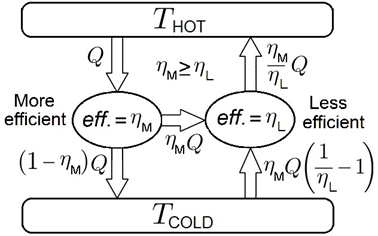
\includegraphics[width=0.5\linewidth]{Lec3/karno_theorem_1}
%	\caption{Доведення першої теореми Карно}
%	\label{pic:karno_theorem_1}
%\end{figure}

\begin{wrapfigure}{R}{0.5\linewidth}
	\centering
	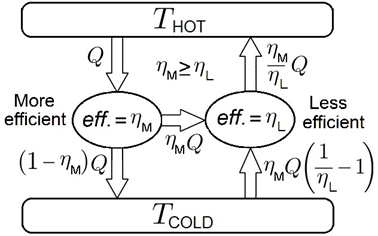
\includegraphics[width=\linewidth]{Lec3/karno_theorem_1}
	\caption{Доведення першої теореми Карно}
	\label{pic:karno_theorem_1}
\end{wrapfigure}

Для доведення теореми розглянемо дві теплові машини М і М', таких що їх К.К.Д. співвідносяться як:
\begin{equation}\label{3.1}
	\eta_M>\eta_L
\end{equation}
при тому, що обидві працюють між температурами $\theta_1$ і $\theta_2$ і виконують рівні роботи $A=\dfrac{\eta_M}{\eta_L}Q$. Із (\ref{3.1}) слідує:
\begin{equation}\label{3.2}
	\eta_M = \dfrac{|A|}{Q} 
\end{equation}
де $Q_1=Q$ та $Q_2=Q'= Q\dfrac{\eta_M}{\eta_L}$  – тепло, отримане від нагрівача машинами М і М', відповідно. Примусимо працювати машину М', як холодильник. Роботу, необхідну для цього, будемо отримувати від машини М. Результатом їх взаємної дії буде:
\begin{enumerate}
	\item [a)] передача в циклі теплоти $\Delta Q = Q' – Q$ від більш холодного тіла до більш гарячого;
	\item [б)] робота не виконується і немає ніяких змін в навколишньому середовищі, що неможливо за формулюванням Клаузіуса.
\end{enumerate}

Такі ж міркування можемо навести припускаючи, що $\eta_L>\eta_M$. Обернувши дію машини, ми знову отримуємо суперечність. Звідси випливає, що $\eta_L = \eta_M$. Зауважимо, що в силу довільності вибору адіабат та робочої речовини, К.К.Д. такої машини від них не залежить. Таким чином К.К.Д. не залежить від параметрів адіабат, а отже є тільки функцією температур нагрівача і холодильника:
\begin{equation}\label{3.3}
	\eta = 1 - \dfrac{Q_2}{Q_1} = f(\theta_1, \theta_2)
\end{equation}

% --------------------------------------------------------
\section{5}
% --------------------------------------------------------

Друга теорема Карно стверджує, що: \emph{К.К.Д. всіх оборотних теплових машин, що мають тепловий контакт з навколишнім середовищем лише при температурах $\theta_1$ і $\theta_2$ становить} $\eta=1-\theta_2/\theta_1$ . Оскільки к.к.д. теплової машини Карно не залежить від робочої речовини і конструкції машини (положення адіабат), для конкретизації виразу К.К.Д. знайдемо його для будь-якого циклу Карно, наприклад для циклу, що працює на ідеальному газі. Користуючись лемою Карно, маємо:
\begin{equation}\label{3.4}
	\eta=1-\dfrac{\theta_2}{\theta_1}
\end{equation}
де $\theta_1$ і $\theta_2$ – значення температур, виміряних емпіричним термометром (наприклад, в ідеальній газовій шкалі).

% --------------------------------------------------------
\section{6}
% --------------------------------------------------------

Відношення (\ref{3.4}) дозволило Томсону (Кельвіну) запропонувати абсолютну  термодинамічну шкалу, тобто такий термометр, покази якого не залежать від природи термометричного тіла. Розглянемо дві теплові машини, що працюють між тепловими резервуарами $\theta_1$ і $\theta_0$ та $\theta_0$ і $\theta_2$, відповідно. $\theta_0$ обираємо довільно, при чому для одної машини резервуар з температурою $\theta_0$ є холодильником, а для іншої нагрівачем. Тоді справедливе відношення
\begin{equation}\label{3.5}
	\dfrac{Q_1}{Q_0} = \phi(\theta_1, \theta_0); ~~ ~~ \dfrac{Q_0}{Q_2} = \phi(\theta_0, \theta_2),
\end{equation}
де $Q_0$ – тепло, віддане в холодильник першою машиною і отримане іншою. Тоді, власне кажучи, проміжний термостат може бути виключений. Для цього перемножимо перше і друге відношення в (\ref{3.5}). Отримаємо
\begin{equation}\label{3.6}
	\dfrac{Q_1}{Q_2} = \phi(\theta_1, \theta_0)\cdot\phi(Q_0,Q_2)
\end{equation}
що еквівалентно
\begin{equation}\label{3.7}
	\phi(\theta_1, \theta_0)\cdot\phi(\theta_0,\theta_2) = \phi(\theta_1, \theta_2)
\end{equation}
У виродженому випадку $\theta_1 = \theta_2$, знайдемо:
\begin{equation}\label{3.8}
	\phi (\theta_1, \theta_0) = \dfrac{1}{\phi(\theta_0, \theta_1)}
\end{equation}
оскільки очевидно, що $\phi(\theta_1,\theta_1)=1$, тобто К.К.Д. циклічного процесу, нагрівачем і холодильником якого є один і той самий тепловий резервуар, дорівнює нулю. Використовуючи (\ref{3.8}), перепишемо (\ref{3.7}) як:
\begin{equation}\label{3.9}
	\phi(\theta_1, \theta_2) = \dfrac{\phi(\theta_1, \theta_0)}{\phi(\theta_2, \theta_0)}
\end{equation}
Але, оскільки в повному циклі Θ0 не фігурує, то: 
\begin{equation}\label{3.10}
	\phi(\theta_1, \theta_2) = \dfrac{\phi(\theta_1)}{\phi(\theta_2)}
\end{equation}
Поклавши тепер, як це було зроблено Томсоном в 1848 році, що $T= \phi(\theta)$ отримуємо:
\begin{equation}\label{3.11}
	\dfrac{Q_1}{Q_2} = \dfrac{T_1}{T_2}
\end{equation}
Це дає принциповий спосіб побудови температурної шкали. Практичний спосіб, що дозволяє пов'язати покази реального термометра $\theta$ із абсолютною температурою $T$, розглянемо згодом. А зараз зазначимо наступні важливі особливості:
\begin{enumerate}
	\item [а)] визначення абсолютної шкали не пов'язано з особливостями термометричного тіла, а визначається лише другим законом термодинаміки;
	\item [б)] гранична температура $T_1=0$ називається абсолютним нулем. Абсолютний нуль існує як математична абстракція, в тому сенсі, що реалізувати цикл Карно з температурою холодильника $T_1=0$ неможливо, оскільки в такому циклі все тепло перетворюється в роботу. Але зауважимо, звідси не витікає неможливість досягнення абсолютного нуля.
	\item [в)] із (\ref{3.11}) випливає, що температура може бути або додатною, або від'ємною.
\end{enumerate}

Довести невід'ємність або від'ємність температури немає можливості. Її знак визначається додатковою домовленістю, яка температура більша, а яка менша. Ми вважаємо, що при передачі тілу за рівноважних умов деякої кількості тепла при фіксованих зовнішніх параметрах, його внутрішня енергія збільшується, що еквівалентно твердженню про невід'ємність теплоємності:
\begin{equation}\label{3.12}
	C_X =\lpdr{U}{T}{X}\geq 0
\end{equation}

% --------------------------------------------------------
\section{7}
% --------------------------------------------------------

Не варто розглядати теплову машину, як деяку машину, придатну лише для виконання корисної роботи. Навпаки, в силу унікальності її властивостей, що слідують із другого закону термодинаміки, наслідки і висновки, отримані при дослідженні її роботи, мають дати нам уявлення про універсальні закономірності, яким слідують термодинамічні системи без винятку. Зокрема, в подальшому тепловою машиною Карно будемо називати будь-який фізичний процес і в будь-якій системі, що виконує цикл Карно.

Розглянемо цикл Карно, утворений безкінечно близькими ізотермами $T$ і $T-\Delta T$. Тепло, отримане від термостату з температурою $Т$ буде: 
\begin{equation}\label{3.13}
	Q_{12} = \left[\lpdr{U}{V}{T} +P\right]\Delta V,
\end{equation}
де $\Delta V$ може бути обрано малим, щоб диференціали можна було замінити приростом, а $\lpdr{U}{V}{T}$ і $Р$ вважати незмінними. З іншого боку робота в циклі, з точністю до малих вищого порядку, дорівнює площі паралелограма 123'4'
\begin{equation}\label{3.14}
	A =\Delta P \Delta V
\end{equation}
Відношення (\ref{3.14}) до (\ref{3.13}) дає К.К.Д. машини Карно:
\begin{equation}\label{3.15}
	\eta = \dfrac{A}{Q_{12}} = \dfrac{\Delta P \Delta V}{\left[\lpdr{U}{V}{T} + P\right]\Delta V} = \dfrac{\Delta T}{T}
\end{equation}
Відношення (\ref{3.15}) тим точніше виконується, чим більш ми \enquote{стягуємо} цикл 1234 в точку 1. Звідси, переходячи до границі, отримаємо
\begin{equation}\label{3.16}
	\lpdr{U}{V}{T} + P = T \lpdr{P}{T}{V}
\end{equation}
Неважко зрозуміти, що отримане співвідношення є універсальним в тому сенсі, що виконується для будь-якої системи, описаної термінами $P$,$V$,$T$, а по-друге, легко може бути узагальнено на інші системи формальною заміною $P\rightarrow F$, а $V\rightarrow x$, де $F$ --- узагальнена сила, а $x$ --- узагальнений зовнішній параметр. Нарешті зауважимо, що в приведеному доведенні добре проглядається взаємозв'язок методу циклів і диференціального підходу Клаузіуса. Почавши з першого, ми зрештою отримаємо диференціальне відношення (\ref{3.16}).

% --------------------------------------------------------
\section{8}
% --------------------------------------------------------

Для безкінечно тонкого циклу Карно, але різниця температур $T_1$  i $T_2$ скінченна, кількість підведеного і відведеного тепла безкінечно мала і тоді
\begin{equation}\label{3.17}
	\dfrac{\delta Q_1}{T_1} = \dfrac{\delta Q_2}{T_2}
\end{equation}
Розглянемо на індикаторній діаграмі довільний фізично можливий цикл\footnote{Суттєво, щоб обраний цикл можна було вкрити сіткою адіабат та ізотерм }. Подаймо увесь процес у вигляді сукупності безкінечно тонких циклів Карно. Для того, щоб це зробити, необхідно, щоб адіабати не перетинались, а ізотерми перетинались з адіабатами лише один раз, що легко доводиться методом циклів з використанням ІІ закону. Між іншим, із перетину  адіабати з ізотермою лише в одній точці можна сформулювати другий закон, як принцип \emph{адіабатичної недосяжності Каратеодорі: \enquote{поблизу будь-якого термічно рівноважного стану термічно однорідної системи існує як завгодно близький інший стан, який ніколи не може бути досягнутий адіабатичним шляхом}}. Для кожного із безкінечно тонких циклів Карно виконується співвідношення (\ref{3.17}). Тоді для суми по всіх циклах це також виконується. В результаті, в границі зубчаста форма покриття циклу зникає, а (\ref{3.17}) переходить в:
\begin{equation}\label{3.18}
	\oint \dfrac{\delta Q }{T} =0.
\end{equation}
Звісно, такий цикл повинен бути оборотним, бо тоді покриття оберненими циклами Карно не буде адекватним. Умова (\ref{3.19}) є необхідною і достатньою умовою існування повного диференціала:
\begin{equation}\label{3.19}
	dS = \dfrac{\delta Q}{T}
\end{equation}
а сама функція $S$ є функцією стану. Неважко побачити, що отримана функція еквівалентна тій, яка була знайдена для ідеального газу і була названа ентропією. В перекладі з грецької ($\epsilon\nu\tau\rho o\pi i \epsilon\nu$) означає здатність до перетворення. Вираз (\ref{3.18}) отримав назву \emph{рівність Клаузіуса} для рівноважних циклічних процесів, а (\ref{3.19}) є фактично математичним змістом другого закону.  Деякі автори так його і формулюють, визначаючи разом із температурою та внутрішньою енергією ще одну функцію стану --- ентропію. По Зоммерфельду: \enquote{\emph{Кожна термодинамічна система має функцію стану названу ентропією. Ентропія розраховується так. Система переводиться із вибраного початкового стану в кінцевий квазістатично; обраховуються при цьому всі підведені до системи порції теплоти $\delta Q$ і діляться на відповідну температуру; всі приведені теплоти підсумовуються}}. 